%Autor: Simon Walker
%Version: 1.0
%Datum: 11.12.2019
%Lizenz: CC BY-NC-SA

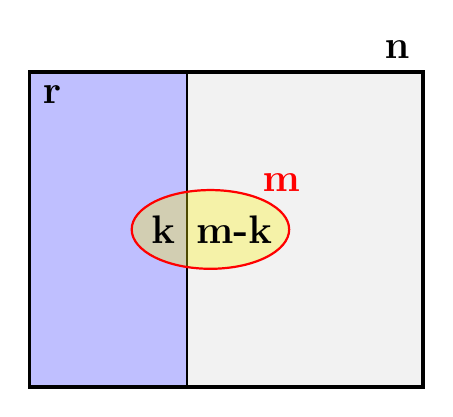
\begin{tikzpicture}
%	\newcommand{\HelpCords}[4]{
%		\draw [help lines] (#1,#2) grid (#3,#4);
%		\foreach \i in {#1,..., #3}
%		\node [below] at (\i,#2) {$\i$};
%		\foreach \i in {#2,..., #4}
%		\node [left] at (#1,\i) {$\i$};
%	}
	
	\filldraw[thick, draw=black, fill=blue!25] (0, 0) rectangle (2, 4);
	\filldraw[thick, draw=black, fill=gray!10] (2, 0) rectangle (5, 4);
	
	\filldraw[thick, draw=red, fill=yellow, fill opacity=.3]
	(2.3, 2) ellipse (1 and 0.5);	
	
	\draw[very thick] (0, 0) rectangle (5, 4);
	
	\Large
	\node[below right] at (0, 4) {\textbf{r}};
	\node[above left] at (5, 4) {\textbf{n}};
	\node at (1.7, 2) {\textbf{k}};
	\node at (2.6, 2) {\textbf{m-k}};
	\node[red] at (3.2, 2.6) {\textbf{m}};
	
	\normalsize
	
%	\HelpCords{0}{0}{5}{4}
\end{tikzpicture}
